
\textbf{a. Mô tả Testbench} 
Chương trình kiểm thử thực hiện phép tính cộng hai số và lưu kết quả vào một địa chỉ đích trong bộ nhớ, gồm các bước:
\begin{itemize}
    \item \textbf{Khởi tạo}: Nạp mã máy của chương trình vào các địa chỉ đầu tiên của RAM.
    \item \textbf{Dữ liệu đầu vào}: Nạp giá trị \texttt{10} (tại địa chỉ \texttt{0x10}) và \texttt{20} (tại địa chỉ \texttt{0x11}).
    \item \textbf{Thực thi lệnh}: 
    \begin{itemize}
        \item \texttt{LDA 0x10}: Nạp giá trị 10 vào thanh ghi Accumulator.
        \item \texttt{ADD 0x11}: Cộng giá trị trong Accumulator với 20, kết quả tạm thời là 30.
        \item \texttt{STO 0x50}: Lưu kết quả (30) từ Accumulator vào địa chỉ bộ nhớ \texttt{0x50}.
        \item \texttt{HLT}: Dừng hệ thống.
    \end{itemize}
    \item \textbf{Kết quả dự tính}: Sau khi tín hiệu \texttt{halt} bật lên, giá trị tại ô nhớ \texttt{0x50} phải bằng \texttt{30}.
\end{itemize}

\textbf{b. Mã nguồn Testbench}

\begin{lstlisting}[language=Verilog, caption={Testbench CPU}]
`timescale 1ns / 1ps

module tb_CPU_System();
    reg clk, rst;
    wire halt;

    CPU_Top uut (.clk(clk), .rst(rst), .halt(halt));

    always #5 clk = ~clk;

    initial begin
        clk = 0; rst = 1;
        
        // Dia chi 0: LDA 0x10 (Opcode 101)
        uut.RAM.ram[0] = {3'b101, 29'h10}; 
        // Dia chi 1: ADD 0x11 (Opcode 010)
        uut.RAM.ram[1] = {3'b010, 29'h11};
        // Dia chi 2: STO 0x50 (Opcode 110)
        uut.RAM.ram[2] = {3'b110, 29'h50};
        // Dia chi 3: HLT (Opcode 000)
        uut.RAM.ram[3] = {3'b000, 29'h0};


        uut.RAM.ram[16] = 32'd10; // Tai dia chi 0x10
        uut.RAM.ram[17] = 32'd20; // Tai dia chi 0x11

        #15 rst = 0;

        wait(halt == 1);
        
        #20;
        $display("Ket qua tai dia chi 0x50: %d", uut.RAM.ram[80]);
        if (uut.RAM.ram[80] == 30) 
            $display("TEST SUCCESSFUL!");
        else 
            $display("TEST FAILED!");
            
        $finish;
    end
endmodule
\end{lstlisting}

\textbf{c. Kết quả xuất ra màn hình} 
\begin{figure}[H]
    \centering
    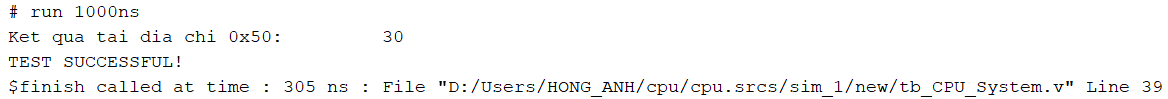
\includegraphics[width=0.8\textwidth]{consolecpu.png} 
    \caption{Kết quả Console thông báo trạng thái kiểm thử hệ thống}
    \label{fig:sys_console}
\end{figure}

\textbf{Đánh giá kết quả:}
\begin{itemize}
    \item \textbf{Luồng thực thi}: CPU thực hiện đúng quy trình Fetch-Decode-Execute cho từng lệnh. 
    Tín hiệu \texttt{halt} bật lên chính xác sau khi hoàn thành lệnh cuối cùng.
    \item \textbf{Độ chính xác dữ liệu}: Phép tính $10 + 20$ được ALU thực hiện chính xác.
    \item \textbf{Tương tác Memory}: Khối Memory đã đáp ứng tốt cả hai vai trò cung cấp mã lệnh và lưu trữ dữ liệu.
    \item \textbf{Kết luận}: Hệ thống tích hợp hoạt động ổn định.
\end{itemize}

\textbf{d. Giản đồ sóng} 

\begin{figure}[H]
    \centering
    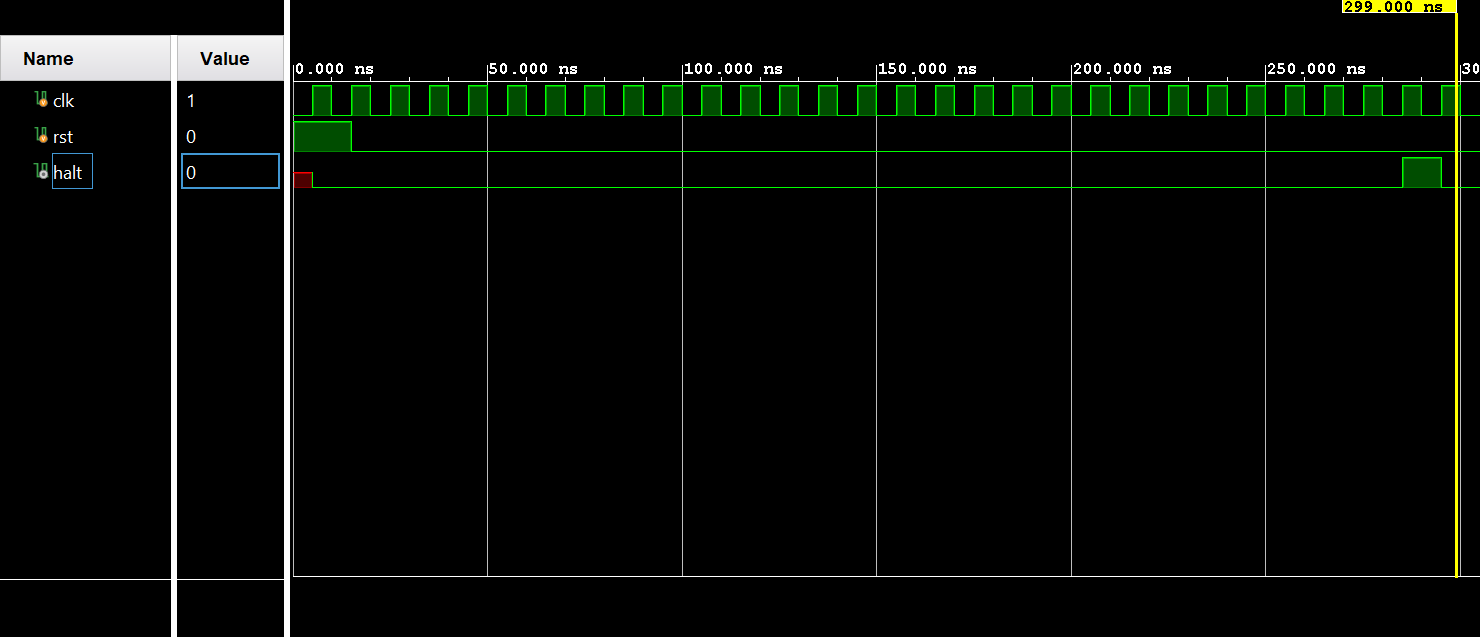
\includegraphics[width=\textwidth]{wavecpu.png} 
    \caption{Giản đồ sóng chương trình tính toán trên hệ thống CPU}
    \label{fig:sys_wave}
\end{figure}

